\documentclass[a4paper,twoside]{article}
\usepackage[T1]{fontenc}
\usepackage[bahasa]{babel}
\usepackage{graphicx}
\usepackage{graphics}
\usepackage{float}
\usepackage[cm]{fullpage}
\pagestyle{myheadings}
\usepackage{etoolbox}
\usepackage{setspace} 
\usepackage{lipsum} 
\usepackage{amsmath}
\usepackage{bm}
\usepackage{subcaption}
\setlength{\headsep}{30pt}
\usepackage[inner=2cm,outer=2.5cm,top=2.5cm,bottom=2cm]{geometry} %margin
% \pagestyle{empty}

\makeatletter
\renewcommand{\@maketitle} {\begin{center} {\LARGE \textbf{ \textsc{\@title}} \par} \bigskip {\large \textbf{\textsc{\@author}} }\end{center} }
\renewcommand{\thispagestyle}[1]{}
\markright{\textbf{\textsc{AIF184001/AIF184002 \textemdash Rencana Kerja Tugas Akhir \textemdash Sem. Ganjil 2026/2027}}}

\newcommand{\HRule}{\rule{\linewidth}{0.4mm}}
\renewcommand{\baselinestretch}{1}
\setlength{\parindent}{0 pt}
\setlength{\parskip}{6 pt}

\onehalfspacing

\begin{document}
	
	\title{\@judultopik}
	\author{\nama \textendash \@npm} 
	
	%tulis nama dan NPM anda di sini:
	\newcommand{\nama}{Vince Farrel Natanael}
	\newcommand{\@npm}{6182301024}
	\newcommand{\@judultopik}{Penerapan MA-Stat-DSM pada Pertandingan Basket} % Judul/topik anda
	\newcommand{\jumpemb}{1} % Jumlah pembimbing, 1 atau 2
	\newcommand{\pembimbing}{Lionov, Ph.D.}
	\newcommand{\tanggal}{22/09/2026}
	
	% Dokumen hasil template ini harus dicetak bolak-balik !!!!
	
	\maketitle
	
	\pagenumbering{arabic}
	
	\section{Deskripsi}

	% Tuliskan deskripsi dari topik tugas akhir yang akan anda ajukan. Di sini dapat dituliskan latar belakang, seperti apa penelitian yang sudah ada sebelumnya dan apa yang akan anda kerjakan. Sertakan gambar agar penjelasan anda menjadi lebih baik.
	% Pada tugas akhir ini, akan dibuat sebuah perangkat lunak yang dapat menampilkan visualisasi dan simulasi kerumunan orang yang berkunjung ke sebuah museum. Dengan menggunakan perangkat lunak tersebut, pengelola museum dapat mengatur tempat peletakan objek sehingga tidak terjadi kerumunan yang terlalu padat.
	
	% Dari berbagai macam teknik yang dapat digunakan untuk melakukan simulasi kerumunan, dipilih dua buah teknik yaitu teknik {\it flow tiles} dan {\it social force model (steering behaviour)}.
	
	% Dst, dst, dst, \ldots\ldots\ldots 
	
	% Perangkat lunak akan dibuat dengan bantuan {\it framework} OpenSteer. Sebagai studi kasus, museum yang digunakan untuk melakukan simulasi adalah Museum Geologi Bandung.
	
	% Dst, dst, dst, \ldots\ldots\ldots 
	
	Manusia sebagai makhluk hidup pasti pernah bergerak.
	Sebagian besar hewan di dunia harus bergerak demi kelangsungan hidupnya, baik untuk melarikan diri dari bahaya maupun untuk mencari makan.
	Manusia tidak ada bedanya, setiap manusia memiliki aspirasi, keinginan, dan tujuan dalam hidup setiap orang, dan untuk manusia dapat mencapai tujuannya, setiap orang harus bergerak menuju tujuan tersebut.
	Setiap hari banyak orang di dunia bergerak untuk mencapai lokasi-lokasi dimana mereka dapat bekerja, belajar, berekreasi, dan lain-lain.
	
	Karena pergerakan merupakan aspek yang sangat penting dalam kehidupan manusia, sepanjang sejarah, orang-orang telah menciptakan berbagai inovasi agar dapat berpindah tempat dengan lebih efisien.
	Upaya manusia dalam meningkatkan efisiensi untuk bergerak sudah dimulai jauh di masa lalu, sejak tahun 4000 BCE dimana manusia sudah mulai menjinakan binatang-binatang seperti kuda hingga 3500 BCE, saat roda pertama ditemukan di Mesopotamia.
	Perkembangan tidak berhenti disana dan terus berlanjut hingga tahun 1814 dimana seseorang bernama George Stephenson membuat mesin uap lokomotif pertama yang memungkinkan perjalanan darat secara massal.
	Lalu juga pada tahun 1886 saat Carl Benz membuat mobil bermesin bensin pertama dan Henry Ford, yang mengotomatisasi perakitan mobil sehingga menjadikannya terjangkau dan lebih mudah diakses.
	Bahkan perkembangan tidak berhenti dalam daratan.
	Pada tahun 1903 sepasang saudara Wilbur dan Orville atau yang lebih dikenalnya atas nama Wright brothers berhasil menaklukan langit untuk pertama kalinya yang membuat yang membantu orang dapat menempuh jarak yang sangat jauh dengan cepat.
	Dan tentunya sekarang, di era modern dimana perkembangan pada teknologi transportasi memperkenalkan teknologi-teknologi seperti kereta cepat dan {\it electric vehicle} atau EVs.

	\begin{figure}[htbp]
		\centering
		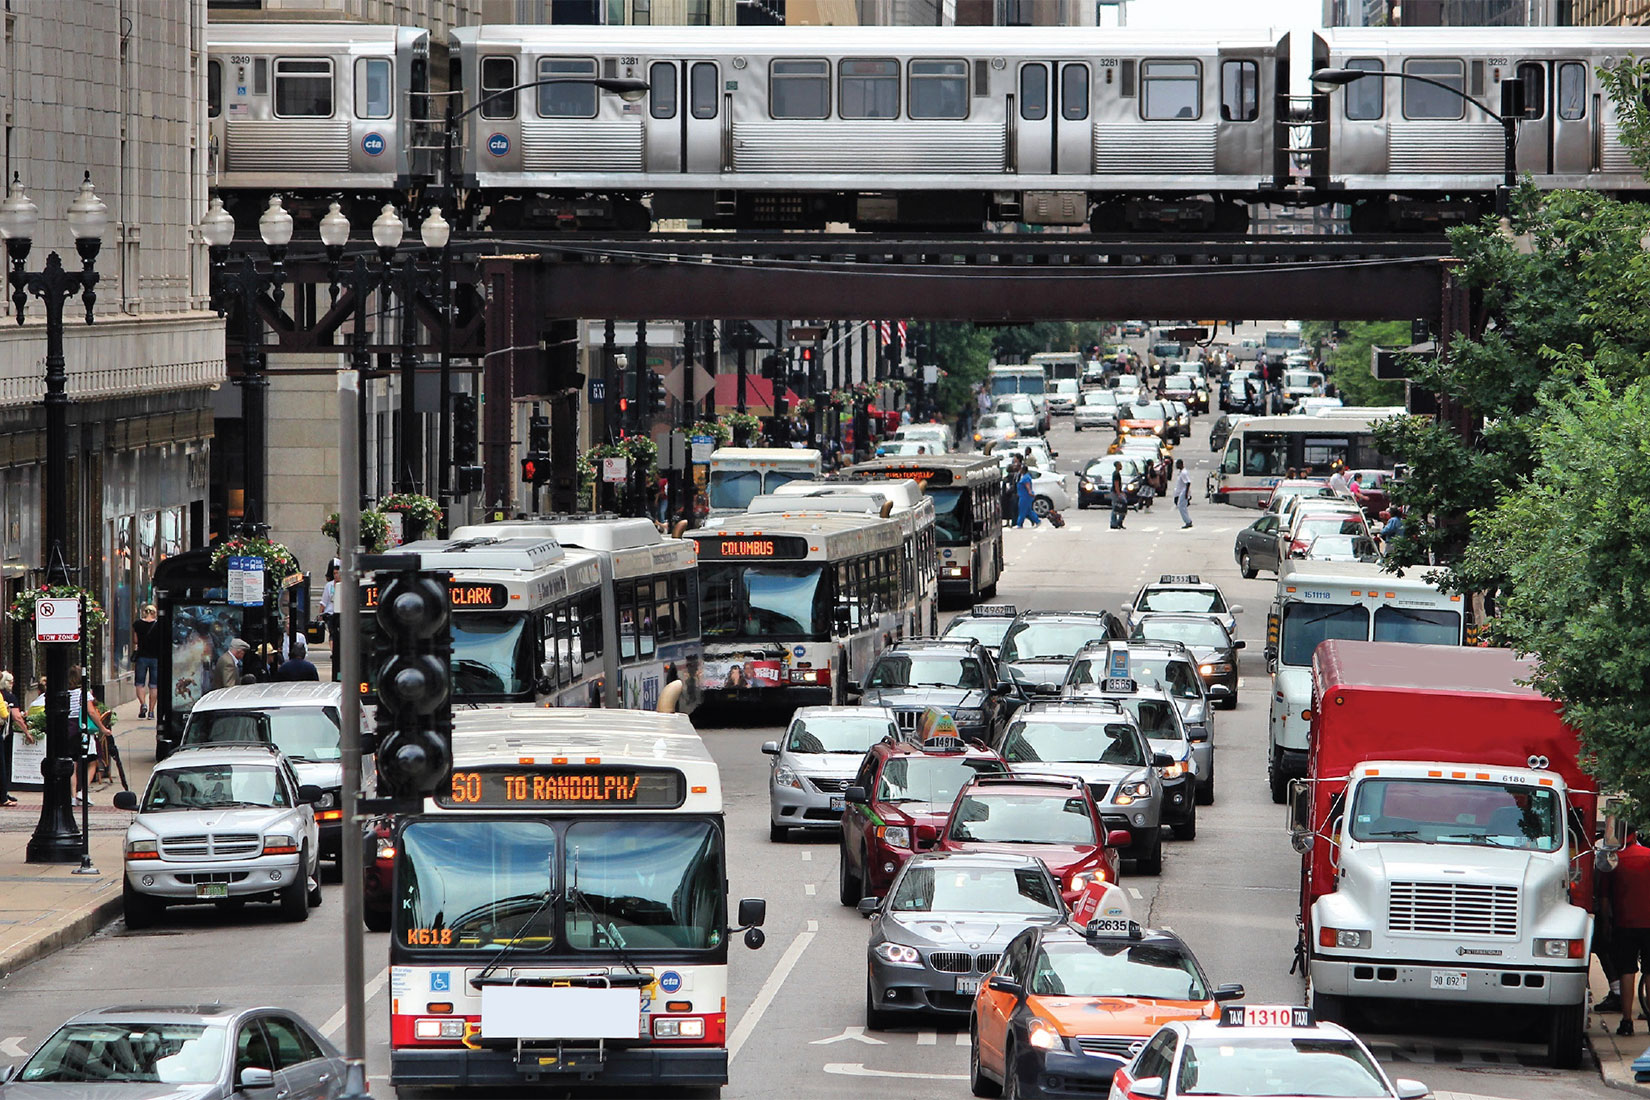
\includegraphics[width=0.5\textwidth]{img/transportation.jpg}
		\caption{Kendaraan buatan manusia}
		\label{fig:man-madeTransportation}
	\end{figure}
	
	Dapat dilihat dari sejarah manusia dan perkembangan teknologi dari zaman dahulu bahwa manusia sangat berupaya untuk memaksimalkan efisiensi pergerakan. Oleh karena itu terdapat banyak ketertarikan dari berbagai orang untuk mempelajari pergerakan-pergerakan yang manusia lakukan. 
	Di zaman modern ini terutama, dikarenakan ketertarikan yang dimiliki banyak orang, perkembangan teknologi pelacakan juga bertumbuh dengan pesat. Dimulai dari saat tahun 1930s-1960s dimana pelacakan hanya dilakukan dengan observasi mata atau fotografi dari udara.
	Dilanjuti ke tahun 1990s-2000s dimana mulai muncul teknologi {\it Global Positioning System} (GPS) yang memudahkan pengambilan dan mengumpulkan data untuk dianalisis.
	Sekarang, di era modern kini, muncul berbagai teknologi baru seperti {\it computer vision} yang mampu mencatat data pergerakan dengan lebih mudah.
	Zaman dahulu, jumlah data pergerakan tidak banyak dan kualitas dari data-data tersebut juga tidak bagus.
	Namun sekarang, karena perkembangan dari teknologi pelacakan menyebabkan lonjakan dalam jumlah dan kualitas data pergerakan.
	Sekarang data pergerakan dapat didapatkan dengan menggunakan lintasan ({\it trajectory}) dari sebuah entitas yang bergerak. 

	Berbeda dengan sebelumnya, teknologi pelacakan seringkali digunakan untuk melacak pergerakan mobil di jalan atau bencana-bencana seperti angin topan, dan lain-lain.
	Namun berkat perkembangan teknologi dalam bidang {\it computer vision} membuat pengumpulan data lintasan di bidang lain jauh lebih mudah dilakukan.
	Salah satu bidang yang terdampak besar dari perubahan ini merupakan pada bidang olahraga dimana sudah banyak diimplementasi oleh berbagai cabang untuk membantu proses pengambilan keputusan.
	Sekarang berbagai organisasi-organisasi dari berbagai cabang olahraga di dunia sudah mulai mengimplementasikan teknologi pengambilan data seperti contohnya olahraga baseball dimana organisasi dengan nama MLB mengambil data lintasan dari bola yang dilempar untuk mendapatkan berbagai informasi seperti kecepatan, putaran, dan lain-lain.
	Atau Tennis dimana organisasi seperti ITF, ATP, WTA menggunakan data lintasan untuk menentukan lokasi bola pada setiap saat.
	Ataupun dalam cabang olahraga sepak bola dimana tidak hanya bola yang dilacak, tetapi juga seluruh pemain-pemain.
	Semua cabang olahraga yang disebutkan tadi dan masih banyak cabang olahraga lainnya telah mengimplementasikan teknologi tersebut untuk membantu mengembangkan kualitas permainan dari cabang olahraga mereka masing-masing.
	
	\begin{figure}[htbp]
		\centering
		\begin{subfigure}[b]{0.45\linewidth}
			\centering
			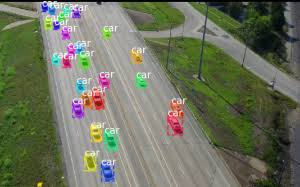
\includegraphics[width=\linewidth]{img/trajectoryCollection.jpg}
			\caption{Pengambilan data lintasan pada kendaraan}
			\label{fig:trajectoryDataCollectionOnVehicle}
		\end{subfigure}
		\hfill 
		\begin{subfigure}[b]{0.45\linewidth}
			\centering
			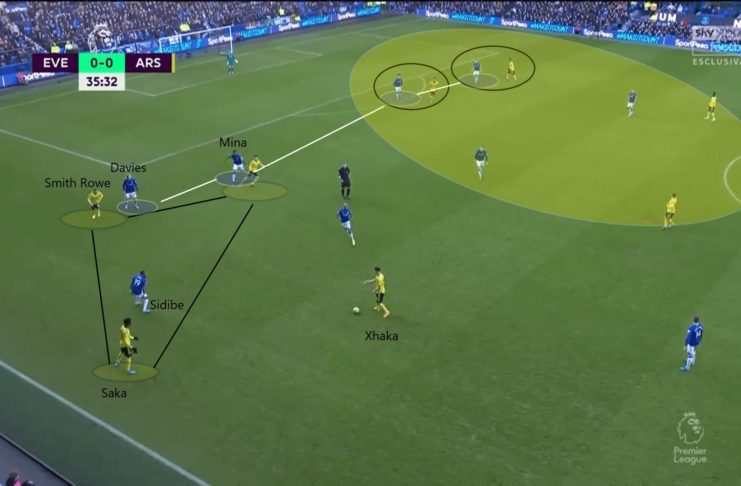
\includegraphics[width=\linewidth]{img/performanceAnalysisOnSoccer.jpg}
			\caption{Analisis performa dalam olahraga sepak bola}
			\label{fig:trajectoryAnalysisOnSoccer}
		\end{subfigure}
		\caption{Penggunaan data lintasan dalam kehidupan}
		\label{fig:examplesOfTrajectoryInTheWorld}
	\end{figure}
	
	Selain untuk pelacakan, terdapat juga berbagai contoh lainnya untuk penggunaan data lintasan. 
	Salah satu penggunaan lainnya untuk data ini adalah untuk analisis yang dapat membantu orang untuk mengambil keputusan berdasarkan hasil analisis tersebut. 
	Beberapa contohnya adalah dalam bidang perencanaan kota dan infrastruktur dimana sebuah riset mengenai penambangan data lintasan dengan Microsoft Research Asia (MSRA) oleh Yu Zheng (2015) memanfaatkan dataset GeoLife dan dataset T-Drive untuk memetakan arus kemacetan, mendeteksi moda transportasi penduduk, serta merencanakan jaringan jalan.
	Ataupun sebuah studi yang dilakukan dari Departemen Transportasi Maryland dengan judul Applications of Trajectory Data From the Perspective of a Road Transportation Agency: Literature Review and Maryland Case Study oleh Nikola Markovic yang menganalisis jutaan titik lintasan GPS untuk meningkatkan keefektifan rute yang diambil bus dan untuk membantu proses merencanakan lokasi pemeliharaan jalan.
	
	Hal yang sama juga sedang terjadi di bidang olahraga pada cabang bola basket. 
	Bola basket merupakan sebuah permainan beregu yang dimainkan oleh dua kelompok masing-masing 5 orang dengan tujuan untuk mencetak poin lebih banyak dari lawan dengan melempar bola kedalam ring yang ditinggikan.
	Permainan bola basket diciptakan pada Desember 1891 oleh Dr. James Naismith di Sekolah Pelatihan YMCA Springfield, Massachusetts, Amerika Serikat merupakan olahraga yang sekarang dimainkan di seluruh dunia oleh lebih dari 600 juta orang di seluruh dunia di lebih dari 200 negara.
	Federasi Bola Basket Dunia (FIBA) didirikan pada tahun 1932 di Jenewa, Swiss berfungsi sebagai induk organisasi international yang berfungsi sebagai induk organisasi internasional yang mengatur, mengawasi, dan mengembangkan olahraga bola basket di seluruh dunia.
	Saat ini, liga bola basket terbesar di dunia adalah National Basketball Association (NBA) yang dibuat pada 3 August, 1949.
	NBA saat ini menampilkan sekitar 30 tim dan pemain-pemain terbaik dari seluruh dunia dan ditonton oleh jutaan orang di seluruh dunia.

	\begin{figure}[htbp]
		\centering
		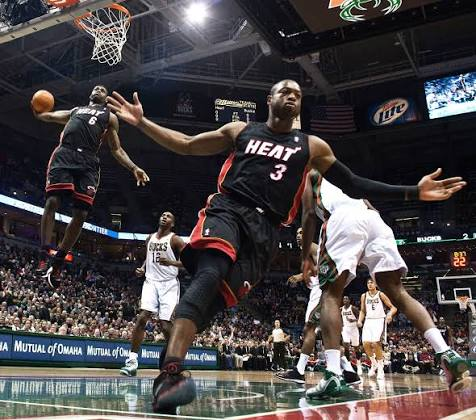
\includegraphics[width=0.5\textwidth]{img/nbaMatch.jpg}
		\caption{Permainan NBA Miami Heats lawan Milwaukee Bucks}
		\label{fig:nba}
	\end{figure}

	Pada sebelum tahun 2000, pengambilan data pada permainan bola basket hanya dapat dilakukan secara manual. 
	Pengambilan data statistik masih dilakukan dengan pencatatan oleh seseorang dari pinggir lapangan dan analisis pertandingan masih dilakukan dengan menonton kembali kaset permainan yang kualitas rekaman masih kurang bagus.
	Baru setelah tahun 2009 bahwa teknologi telah berkembang cukup untuk rekaman pertandingan dapat dilakukan dengan menggunakan peralatan optik seperti kamera yang menyediakan kualitas rekaman yang bagus.
	Berkat kemajuan teknologi ini, peneliti-peneliti mulai dapat menghasilkan data-data lintasan yang memadai.
	Data-data tersebut kemudian digunakan untuk berbagai kebutuhan-kebutuhan baru seperti menganalisis kecepatan lari atau area tembak.
	Data dihasilkan dengan menaruh berbagai kamera yang menangkap seluruh permainan dan merekam semua pemain.
	Dan di era digital sekarang dimana terdapat banyak metode analisis baru yang dibuat untuk menganalisis data tersebut.

	{\it Trajectory} atau lintasan merupakan sebuah jalur yang kontinu yang dilalui oleh suatu entitas yang bergerak dari satu titik ke titik yang lain dalam suatu rentang waktu.
	Dalam sebuah lintasan, dapat dibagi lagi menjadi sub-lintasan yang merupakan bagian dari lintasan dalam rentan waktu tertentu yang merupakan bagian dari rentang waktu keseluruhan lintasan tersebut dan juga bersifat kontinu.
	Karena keterbatasan teknologi, lintasan yang didapatkan tidak bisa benar-benar bersifat kontinu.
	Hal ini dikarenakan teknologi yang digunakan seringkali hanya dapat mencatat lokasi entitas setiap interval waktu tertentu.

	Data lintasan yang digunakan berupa spatio-temporal tracking data yang terdiri atas dua komponen utama.
	Komponen yang pertama terdiri dari data spatio yaitu data lokasi sebuah atau beberapa entitas dalam bidang dua atau tiga dimensi dan untuk komponen kedua merupakan data temporal yaitu data waktu dimana entitas tersebut berada di suatu lokasi.
	Kedua komponen tersebut saat disatukan membentuk data yang dapat menjelaskan dimana suatu entitas berada pada suatu waktu tertentu.
	Dengan jumlah yang banyak dan dengan waktu yang kontinu, dapat digabung dan menjadi data lintasan entitas tersebut yang memperlihatkan pergerakan entitas tersebut.

	\begin{figure}[htbp]
		\centering
		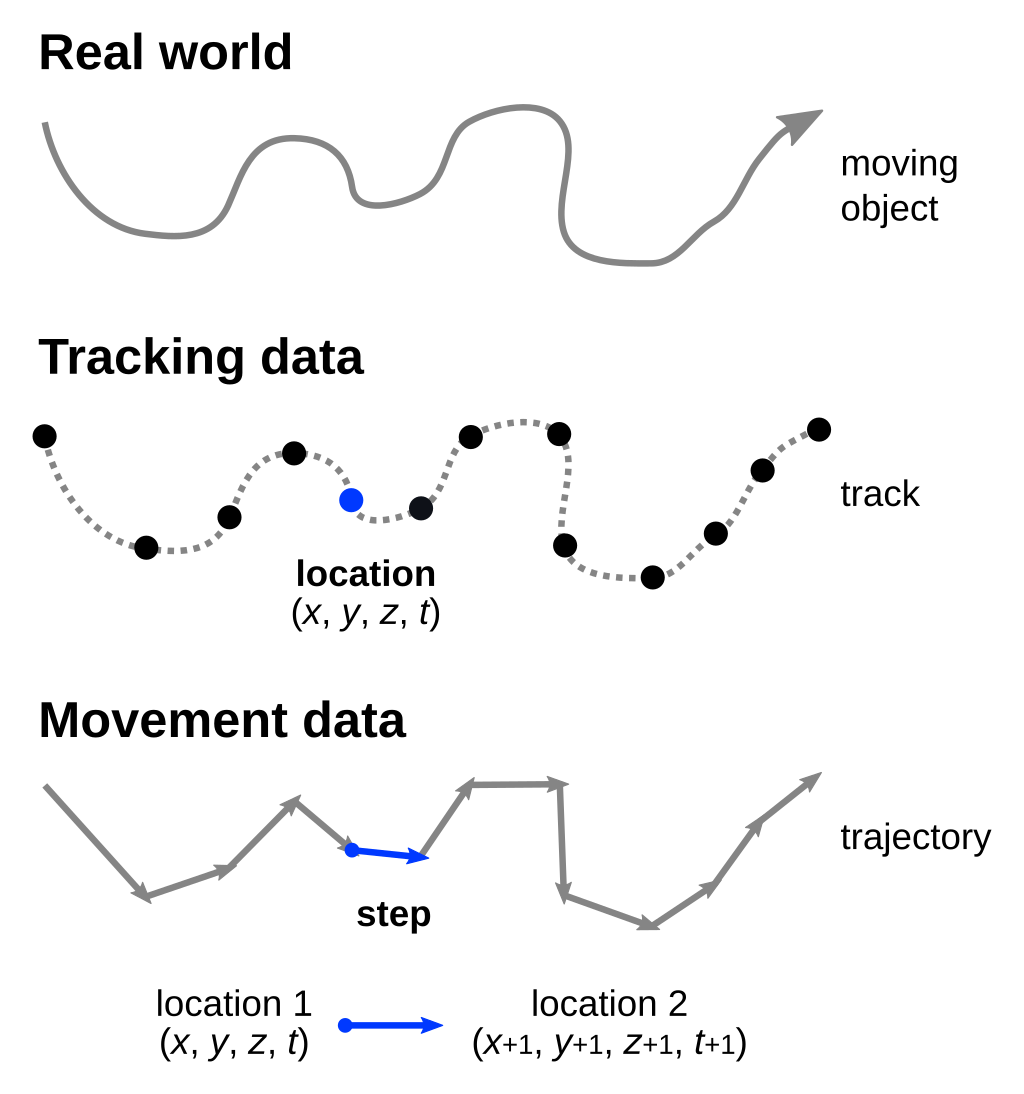
\includegraphics[width=0.5\textwidth]{img/trajectoryExplanation.png}
		\caption{Perbedaan pergerakan pada dunia nyata (Real world) yang bersifat kontinu dengan data pelacakan (Tracking data) yang dicatat hanya pada waktu tertentu sehingga membentuk rangkaian titik yang disebut pelacakan dan data pergerakan (Movement data) yang direpresentasikan dengan kumpulan langkah-langkah dari satu lokasi ke lokasi lain yang membentuk suatu lintasan}
		\label{fig:trajectoryExplanation}
	\end{figure}

	Salah satu dataset untuk data lintasan pertandingan basket yang banyak digunakan adalah dataset yang disediakan oleh SportVU.
	SportVU merupakan sebuah sistem kamera yang tujuan utamanya adalah untuk mengikuti bola dan pemain-pemainnya pada lapangan.
	SportVU menyediakan statistik seperti posisi pemain dan bola secara waktu nyata melalui perangkat lunak dan algoritma statistik.

	Seiring dengan perkembangan teknologi pengambilan data lintasan seperti penggunaan SportVU, dibuat juga berbagai metode untuk memproses data-data yang dikumpulkan.
	Salah satu contoh penggunaan dari data lintasan dari SportVU tersebut untuk dianalisis oleh komputer untuk dibandingkan dengan permainan-permainan lainnya untuk menentukan apakah sebauh serangan dapat dianggap efektif atau tidak.
	Dengan ini, permainan bola basket dapat semakin dalam dimengerti untuk perkembangan pemain dan juga pelatih-pelatih dalam merancang startegi serangan untuk tim mereka.
	Hasil analisis yang didapatkan dari komputer dapat kemudian dianalisis lagi lebih lanjut oleh pelatih-pelatih tim basket untuk kemudian mereka dapat merancang pelatihan atau strategi baru untuk tim mereka.
	Hasil analisis juga bisa juga dipakai oleh tim musuh untuk melihat serangan mana yang terlihat efektif dan bisa antara merancang pertahanan terhadap strategi tersebut atau dapat merancang startegi serangan berdasarkan analisis tersebut.

	Salah satu penelitian yang menggunakan SportVU dalam cabang bola basket adalah studi {\it Multi-agent statistical discriminative sub-trajectory mining and an application to NBA basketball} oleh Bunker et al.(2023). 
	Pada studi tersebut, Rory Bunker menggunakan dataset SportVU dari tahun 2015 dan 2016 untuk dianalisis.
	Studi tersebut menggunakan sebuah metode dengan nama Multi Agent Statistically Discriminative Sub-Trajectory Mining (MA-Stat-DSM) untuk membandingkan sebuah serangan terhadap serangan-serangan lainnya dan menentukan keefektifan serangan tersebut.
	Salah satu hasil yang didapat dari analisis adalah pada salah satu serangan yang dilakukan oleh Golden State Warriors melawan Los Angeles Lakers pada 5 Januari 2016, model berhasil mengidentifikasi serangan yang effisien yang menunjukan pergerakan shooter yang lebih cepat dibandingkan defender yang menghasilkan shooter dapat bergerak ke tepi setengah lingkaran dan menerima bola dan melakukan tembakan kosong.

	\begin{figure}[H]
		\centering
		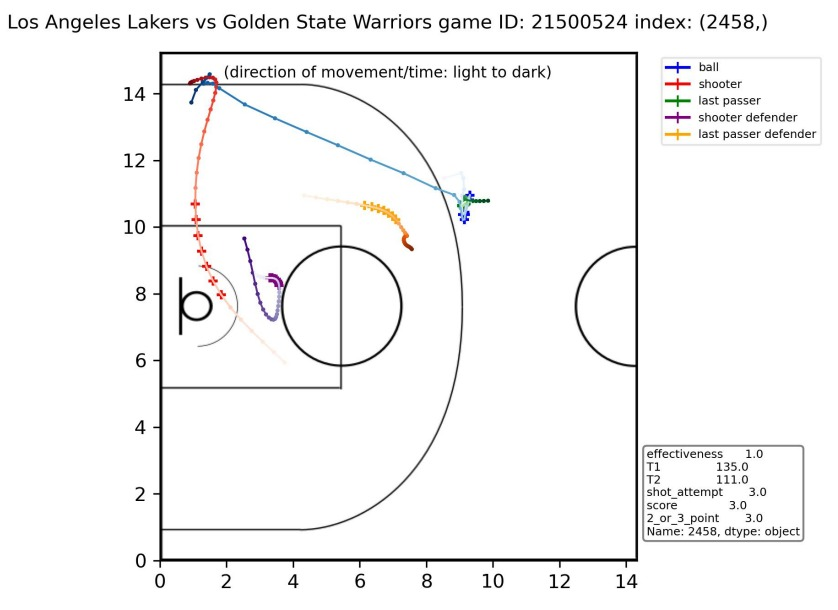
\includegraphics[width=0.7\textwidth]{img/GSWvLakers.jpeg}
		\caption{Grafik serangan efektif dari Golden State Warriors melawan LA Lakers}
		\label{fig:GSWvLakersGraph}
	\end{figure}

	Untuk dataset yang digunakan, dataset SportVU berisi dengan informasi pertandingan antara dua tim dan juga berisi informasi pemain pada kedua tim.
	Informasi pemain pada SportVU mencakup informasi tim yang ditampilkan melalui ID tim, jenis tim (tuan rumah atau tamu), nama tim, dan singkatan nama tim serta informasi pemain yang ditampilkan melalui ID pemain, nama depan dan belakang pemain, nomor punggung, dan posisi bermain (G - Guard, F - Forward, C - Center).
	Informasi permainan tersedia dalam bentuk data pelacakan yang dibagi berdasarkan waktu, di mana setiap satuan waktu kemudian dirinci lagi untuk setiap pemain. Setiap pengukuran memuat informasi mengenai {\it event ID}, nomor babak, {\it timestamp}, waktu permainan ({\it game clock} dan {\it shot clock}), {\it team ID} dan {\it player ID}, serta lokasi pemain dalam koordinat xyz. 
	Terdapat pula pengukuran untuk bola, yang ditandai dengan nilai -1 pada {\it team ID} dan {\it player ID}.

	\begin{figure}[htbp]
		\centering
		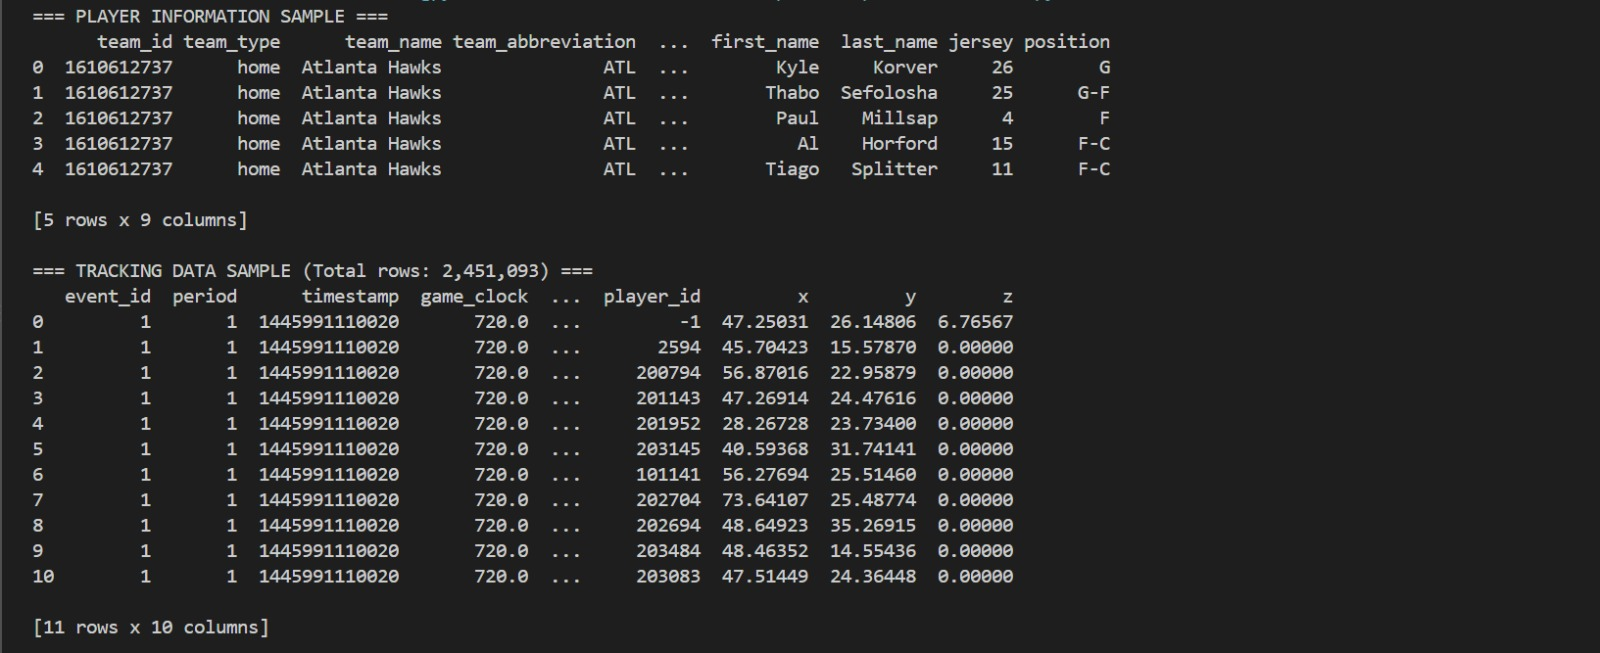
\includegraphics[width=1\textwidth]{img/SportVUData.jpeg}
		\caption{Data yang didapatkan dari dataset SportVU}
		\label{fig:sportvudata}
	\end{figure}

	Sebelum membicarakan MA-Stat-DSM, pertama harus dibicarakan mengenai apa itu metode Statistically Discriminative Sub-Trajectory Mining (Stat-DSM).
	Stat-DSM merupakan metode untuk menganalisis data lintasan spatio-temporal dengan tujuan untuk menemukan pola-pola dari pergerakan suatu entitas.
	Stat-DSM menganalisis sub-lintasan dari sebuah lintasan entitas dan melihat apakah pola-pola pergerakan dalam sub-lintasan.
	Sub-lintasan tersebut kemudian ditempatkan ke dalam salah satu kelompok berdasarkan karateristik-karateristik pergerakannya.
	Sub-lintasan akan dianggap sebagai diskriminatif hanya bila sub-lintasan tersebut serupa dengan banyak sub-lintasan lainnya dalam suatu kelompok dan tidak serupa dengan (atau hanya serupa dengan sedikit) lintasan dalam kelompok lain.	

	\begin{figure}[htbp]
		\centering
		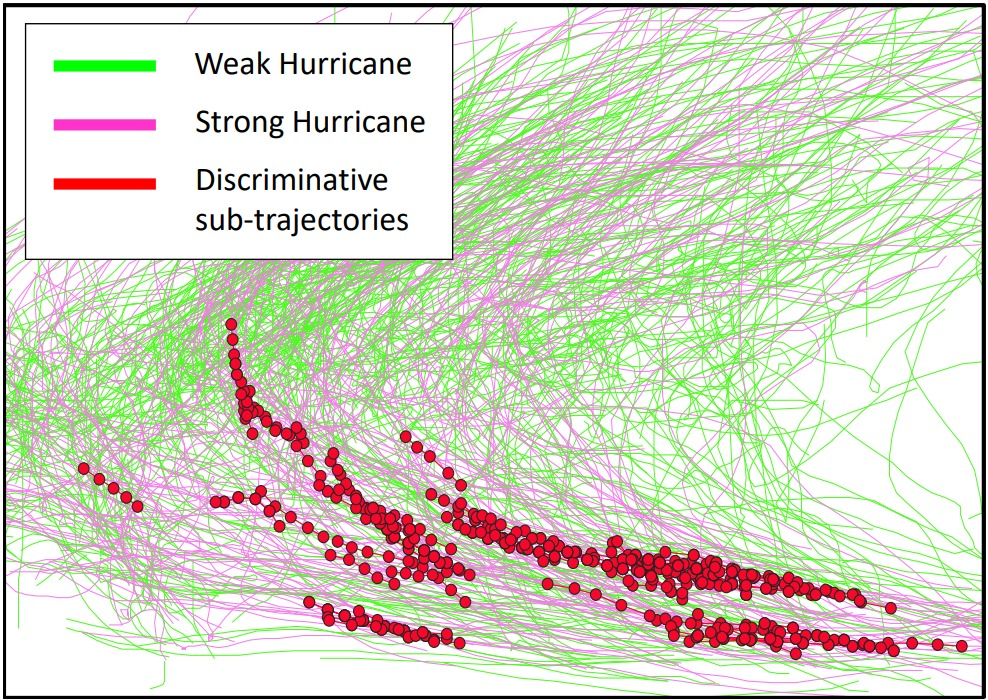
\includegraphics[width=0.5\textwidth]{img/StatDSMTrajectory.jpeg}
		\caption{Data lintasan pada angin topan}
		\label{fig:trajectoryOnHurricane}
	\end{figure}

	Metode Stat-DSM sudah dipakai dalam menganalisis data lintasan dari berbagai entitas seperti angin topan atau kendaraan di jalan.
	Namun, untuk bidang dimana terdapat banyak entitas seperti dalam permainan olahraga beregu, metode ini tidak dapat diimplementasi semudah itu.
	Dapat secara naif digunakannya metode Stat-DSM, dengan cara menggunakan metode tersebut dalam seluruh data lintasan setiap agen.
	Tetapi dengan menggunakan metode ini, terdapat kemungkinan akan adanya kehilangan informasi spatio-temporal yang penting dalam interaksi antar agen dan juga daya komputasi dan waktu yang diperlukan untuk menganalisis data juga lebih besar.
	
	Oleh karena itu diperlukannya metode lain yang memiliki kapabilitas untuk menganalisis data lintasan dari berbagai agen (pemain dan bola) dan untuk dapat mempertimbangkan interaksi dari beberapa sub-lintasan terhadap sub-lintasan lainnya dalam waktu yang bersamaan.
	Diperlukannya metode untuk menganalisa sub-lintasan secara kolektif dari beberapa entitas di saat yang bersamaan.
	Oleh karena itu, dibuatnya metode lain yaitu metode Multi-Agent Statistically Discriminative Sub-Trajectory Mining, yaitu metode pengembangan dari Stat-DSM.
	Dengan menggunakan metode ini, pertandingan basket akan dapat dianalisis dengan lebih dalam dan interaksi antar sub-lintasan antar agen juga dapat lebih dalam dipelajari.
	Menggunakan metode MA-Stat-DSM, kesimpulan yang didapatkan akan dalam dibandingkan dengan menggunakan analisis statistik konvensional.

	Multi-Agent Statistically Discriminative Sub-Trajectory Mining (MA-Stat-DSM) adalah sebuah metode yang dibuat dengan tujuan untuk dapat mengidentifikasi sub-matriks diskriminatif yang secara statistik bersifat signifikan.
	Di dalam sub-matrix tersebut adalah sub-lintasan dari agen-agen yang ditentukan.
	Metode Stat-DSM bekerja dengan cara menganalisis vektor-vektor yang isinya merupakan kumpulan informasi lokasi yang diurut berdasarkan waktu yang saat digabungkan membentuk sebuah sub-lintasan.
	Perkembangan dari Stat-DSM dan MA-Stat-DSM berada di analisis yang dilakukan dimana Stat-DSM menganalisis vektor yang berisi data lintasan sebuah entitas, MA-Stat-DSM menganalisis sub-matriks yang isi dari matriks merupakan vektor-vektor dengan isi data lintasan dari beberapa agen.

	% Pada MA-Stat-DSM, lintasan $T_{i,k}$ pada matrix $i$ terdiri dari $m_i$ buah data lintasan dari agen $k$ yang dinotasikan dengan \[ T_{i,k} = \{(x_{1,k}, y_{1,k}), (x_{2,k}, y_{2,k}), \dots, (x_{m_i,k}, y_{m_i,k})\} \]
	% Matrik lintasan $i$ memuat semua lintasan dari $K$ agen dalam sebuah serangan, memiliki $m_i$ kolom dan dinotasikan sebagai $\bm{T}_{i,K}$.
	% Terdapat $N$ buah matriks lintasan dalam setiap pertandingan $M$.
	% Setiap matriks lintasan mengambil label $g_i = \{+1,-1\}$, dan $G_+ = \{\bm{T}_{i,K}\ |\ g_i = +1\}$ dan $G_- = \{\bm{T}_{i,K}\ |\ g_i = -1\}$.
	% Label tersebut menandakan apakah serangan yang direpresentasikan oleh matriks lintasan tersebut dianggap "efektif" atau "tidak efektif"

	% Sub-matriks lintasan dinotasikan dengan $\bm{T}_{i,K}^{(s,e)}$ merupakan sebuah urutan kolom dari matriks lintasan $\bm{T}_{i,K}$ yang dimulai dari kolom $s$ dan diakhiri dengan kolom $e$ dengan jumlah baris $|K|$ yang tetap.
	% Setiap sub-matriks $i$ memiliki panjang $|\bm{T}_{i,K}^{(s,e)}| \ge L$, dimana $L$ adalah parameter yang ditetapkan sebelumnya oleh pengguna yang menandakan panjang minimum (jumlah kolom minimum) dari sub-matriks lintasan.
	% Sub-matriks lintasan dinotasikan dengan $\bm{T}_{i,K}^{(s,e)} \sqsubseteq \bm{T}_{i,K}$ yang menandakan bahwa $\bm{T}_{i,K}^{(s,e)}$ merupakan sub-matriks lintasan dari $\bm{T}_{i,K}$.

	Untuk pengerjaan tugas akhir ini akan digunakannya juga metode MA-Stat-DSM buatan Bunker et al. untuk menganalisis pertandingan bola basket. 
	Metode tersebut akan digunakan untuk menganalisis data permainan dari berbagai pertandingan dari berbagai dataset-dataset lain.
	Tidak juga ditutup kemungkinannya untuk dilakukannya penyesuaian-penyesuaian terhadap algoritma MA-Stat-DSM.
	Perangkat lunak akan menerima {\it input} berupa data lintasan beberapa agen dari dataset-dataset yang disediakan.
	Data lintasan akan berupa kumpulan koordinat yang diurut secara waktu untuk membentuk lintasan.
	Pengeluaran dari perangkat lunak akan berupa statistik yang isinya adalah matriks sub-lintasan yang merepresentasikan suatu serangan dengan label yang mendandakan apakah matriks tersebut diskriminative yang signifikan secara statistik atau tidak yang kemudian akan dapat dianalisis lanjut oleh orang untuk menarik kesimpulan mereka sendiri. 
	Perangkat lunak akan dibuat dengan bahasa python menggunakan berbagai library sesuai kebutuhan.

	\section{Rumusan Masalah}
	% Tuliskan rumusan dari masalah yang akan anda bahas pada tugas akhir ini. Rumusan masalah biasanya berupa kalimat pertanyaan. Gunakan penomoran untuk menuliskan rumusan masalah ini.
	
	\begin{enumerate}
		\item Bagaimana menerapkan metode MA-Stat-DSM pada data lintasan pemain pada suatu pertandingan bola basket?
		\item Pola sub-lintasan seperti apa yang dapat ditemukan pada data lintasan pemain bola basket, dan bagaimana interpretasinya dalam konteks permainan?
		\item Modifikasi dalam bentuk apa yang dapat dilakukan terhadap algoritma MA-Stat-DSM untuk meningkatkan hasil eksperimen pada data lintasan pemain bola basket?
		\item Bagaimana kinerja MA-Stat-DSM yang telah dimodifikasi berdasarkan hasil eksperimen pada data lintasan pemain bola basket?
	\end{enumerate}

	\section{Tujuan}
	% Tuliskan tujuan dari topik tugas akhir yang anda ajukan. Tujuan penelitian biasanya berkaitan erat dengan pertanyaan yang diajukan di bagian rumusan masalah. Gunakan penomoran untuk menuliskan rumusan masalah ini, di mana tiap nomor berkaitan dengan nomor pada rumusan masalah.
	
	\begin{enumerate}
		\item Mengimplementasikan metode MA-Stat-DSM untuk menganalisis data lintasan pemain pada pertandingan bola basket. 
		\item Mengidentifikasi pola sub-lintasan yang ditemukan pada data lintasan pemain bola basket serta menginterpretasikan pola tersebut dalam konteks pertandingan bola basket.
		\item Merancang dan menerapkan modifikasi pada algoritma MA-Stat-DSM untuk memperolah hasil eksperimen yang lebih baik.
		\item Mengevaluasi kinerja algoritma MA-Stat-DSM yang telah dimodifikasi berdasarkan hasil eksperimen pada data lintasan pemain bola basket.
	\end{enumerate}

	\section{Deskripsi Perangkat Lunak}
	% Tuliskan deksripsi dari perangkat lunak yang akan anda hasilkan. Apa saja fitur yang disediakan oleh PL tersebut dan apa saja kemampuan dari PL tersebut. Perhatikan contoh di bawah ini:
	
	Perangkat lunak akhir yang akan dibuat memiliki fitur minimal sebagai berikut:
	% \begin{itemize}
	% 	\item Pengguna dapat melihat denah Musem Geologi Bandung dalam bidang dua dimensi. Sedangkan pengunjung direpresentasikan menggunakan lingkaran-lingkaran kecil (tidak menggunakan gambar manusia yang diambil dari atas)
	% 	\item Pengguna dapat memunculkan atau menghilangkan gambar {\it flow tiles} pada denah museum. 
	% 	\item Pengguna dapat mengatur jalannya simulasi: memulai(start) simulasi, menunda(pause) simulasi, melanjutkan(continue) simulasi, maupun menghentikan(stop) simulasi
	% 	\item Pengguna dapat mengatur banyaknya pengunjung di dalam museum, baik melalui perubahan frekuensi kedatangan pengunjung maupun menambahkan dan menghapus pengunjung satu-persatu secara manual.
	% 	\item Posisi kamera dapat diubah (pergerakan di bidang tiga dimensi) sehingga pengguna dapat melihat simulasi di museum dari berbagai arah. 
	% 	\item Posisi kamera dapat diubah untuk emngikuti perjalanan seorang pengunjung di dalam 
	% 	\item Pengguna dapat memilih apakah akan menggunakan teknik {\it flow tiles} atau tidak pada saat simulasi berlangsung
	% 	\item Jenis {\it flow tiles} yang digunakan dapat diubah-ubah pada saat simulasi sedang berlangsung
	% \end{itemize}

	\begin{itemize}
		\item Pengguna dapat memasukkan data pertandingan basket yang berisi dengan informasi lintasan pemain dan bola basket serta waktunya.
		\item Pengguna dapat memilih bagian mana pada data pertandingan yang diberikan untuk dianalisis oleh model.
		\item Program dapat memodelkan pergerakan pemain dan bola berdasarkan data lintasan dan sub-lintasan yang dipilih oleh pengguna.
		\item Program dapat menerapkan model MA-Stat-DSM untuk untuk mencari karateristik-karateristik diskriminan secara statistik dalam sub-lintasan yang dipilih.
		\item Program dapat membuat kesimpulan serangan berdasarkan analisis yang telah dilakukan.
		\item Program dapat memberikan hasil analisis dan menampilkannya dengan cara yang mudah dimengerti pengguna
		\item Program menyediakan opsi untuk pengaturan hyperparameter. 
	\end{itemize}
	
	\section{Detail Pengerjaan Tugas Akhir}
	% Tuliskan bagian-bagian pengerjaan skripsi secara detail. Bagian pekerjaan tersebut mencakup awal hingga akhir skripsi, termasuk di dalamnya pengerjaan dokumentasi skripsi, pengujian, survei, dll.
	
	Bagian-bagian pekerjaan skripsi ini adalah sebagai berikut :
	% \begin{enumerate}
	% 	\item Melakukan survei ke Museum Geologi Bandung untuk mendapatkan denah serta mengetahui perilaku pengunjung museum secara umum (arah perjalanan, kecepatan, lama melihat objek, dll)
	% 	\item Melakukan analisis pada hasil survei terhadap pergerakan pengunjung di museum dan membuat rancangan denah di komputer yang dilengkapi dengan penghalang dan objek di museum.
	% 	\item Melakukan studi literatur mengenai sifat kolektif suatu kerumunan, teknik {\it social force model} dan teknik {\it flow tiles}
	% 	\item Mempelajari bahasa pemrograman C++ dan cara menggunakan framework OpenSteer
	% 	\item Merancang pergerakan kerumunan di dalam museum menggunakan teknik {\it social force model} dan {\it flow tiles} serta menggunakan teknik lainnya seperti konsep pathway dan waypoints. Selain itu, dirancang pula adanya waktu tunggu (pada saat pengunjung melihat objek di museum) dan cara pembuatan jalur bagi setiap individu pengunjung
	% 	\item Melakukan analisa dan merancang struktur data yang cocok untuk menyimpan penghalang (obstacle)
	% 	\item Mengimplementasikan keseluruhan algoritma dan struktur data yang dirancang, dengan menggunakan framework OpenSteer 
	% 	\item Melakukan pengujian (dan eksperimen) yang melibatkan responde untuk menilai hasil simulasi secara kualitatif
	% 	\item Menulis dokumen tugas akhir.
	% \end{enumerate}

	\begin{enumerate}
		\item Mempelajari secara mendalam mengenai konsep Machine Learning, Deep Learning, dan Data Mining.
		\item Melakukan studi literatur mengenai lintasan serta dataset yang digunakan dan bagaimana cara untuk menganalisanya.
		\item Mempelajari dan menguasai metode MA-Stat-DSM serta memahami konsep-konsep lainnya yang berhubungan.
		\item Mempelajari bahasa pemrograman python dan {\it library} yang hendak digunakan. 
		\item Merancang startegi pra-pemrosesan untuk data yang digunakan.
		\item Menganalisa dan memodelkan data lintasan pemain dan fitur-fitur lainnya yang bersifat diskriminatif yang dapat memberikan informasi mengenai pergerakan kedua tim dan entitas lainnya yang berhubungan.
		\item Implementasi metode MA-Stat-DSM dengan menggunakan bahasa pemrograman python.
		\item Melakukan pengujian dengan dataset yang tersedia untuk menilai kinerja model.
		\item Mempersiapkan dokumentasi program yang lengkap.
		\item Mempersiapkan dokumen tugas akhir. 
	\end{enumerate}
	
	\section{Rencana Kerja}
	Rincian capaian yang direncanakan di Tugas Akhir 1 adalah sebagai berikut:
	\begin{enumerate}
		\item Melakukan studi literatur secara mendalam mengenai konsep Machine Learning, Deep Learning, dan Data Mining.
		\item Melakukan studi literatur mengenai lintasan dan data set yang digunakan.
		\item Mempelajari penggunaan bahasa python.
		\item Mempelajari dan memahami library yang hendak digunakan.
		\item Menyusun dokumen laporan Tugas Akhir 1.
	\end{enumerate}
	
	Sedangkan yang akan diselesaikan di Tugas Akhir 2 adalah sebagai berikut:
	\begin{enumerate}
		\item Merancang strategi pra-pemrosesan untuk datase yang digunakan.
		\item Menganalisa dan memodelkan dataset dan menentukan fitur-fitur yang dianalisa.
		\item Implementasi metode MA-Stat-DSM.
		\item Melakukan pengujian model.
		\item Mempersiapkan dokumentasi dari perangkat lunak.
		\item Menyusun dokumen laporan Tugas Akhir 2.
	\end{enumerate}
	
	\vspace{1cm}
	\centering Bandung, \tanggal\\
	\begin{figure}[htbp]
		\centering
		
\includegraphics[width=0.3\textwidth]{img/TTDVinceF.jpeg}
		\label{fig:ttdVinceF}
	\end{figure}
	\nama \\ 
	\vspace{1cm}
	
	Menyetujui, \\
	\ifdefstring{\jumpemb}{2}{
		\vspace{1.5cm}
		\begin{centering} Menyetujui,\\ \end{centering} \vspace{0.75cm}
		\begin{minipage}[b]{0.45\linewidth}
			% \centering Bandung, \makebox[0.5cm]{\hrulefill}/\makebox[0.5cm]{\hrulefill}/2013 \\
			\vspace{2cm} Nama: \makebox[3cm]{\hrulefill}\\ Pembimbing Utama
		\end{minipage} \hspace{0.5cm}
		\begin{minipage}[b]{0.45\linewidth}
			% \centering Bandung, \makebox[0.5cm]{\hrulefill}/\makebox[0.5cm]{\hrulefill}/2013\\
			\vspace{2cm} Nama: \makebox[3cm]{\hrulefill}\\ Pembimbing Pendamping
		\end{minipage}
		\vspace{0.5cm}
	}{
		% \centering Bandung, \makebox[0.5cm]{\hrulefill}/\makebox[0.5cm]{\hrulefill}/2013\\
		\vspace{2cm} Nama: \pembimbing\\\ Pembimbing Tunggal
	}
\end{document}